\documentclass[a4paper]{book}
\usepackage{a4wide}
\usepackage{makeidx}
\usepackage{graphicx}
\usepackage{multicol}
\usepackage{float}
\usepackage{listings}
\usepackage{color}
\usepackage{textcomp}
\usepackage{alltt}
\usepackage{times}
\usepackage{ifpdf}
\ifpdf
\usepackage[pdftex,
            pagebackref=true,
            colorlinks=true,
            linkcolor=blue,
            unicode
           ]{hyperref}
\else
\usepackage[ps2pdf,
            pagebackref=true,
            colorlinks=true,
            linkcolor=blue,
            unicode
           ]{hyperref}
\usepackage{pspicture}
\fi
\usepackage[utf8]{inputenc}
\usepackage{doxygen}
\lstset{language=C++,inputencoding=utf8,basicstyle=\footnotesize,breaklines=true,breakatwhitespace=true,tabsize=8,numbers=left }
\makeindex
\setcounter{tocdepth}{3}
\renewcommand{\footrulewidth}{0.4pt}
\begin{document}
\hypersetup{pageanchor=false}
\begin{titlepage}
\vspace*{7cm}
\begin{center}
{\Large Reference Manual}\\
\vspace*{1cm}
{\large Generated by Doxygen 1.6.3}\\
\vspace*{0.5cm}
{\small Mon Feb 28 13:45:05 2011}\\
\end{center}
\end{titlepage}
\clearemptydoublepage
\pagenumbering{roman}
\tableofcontents
\clearemptydoublepage
\pagenumbering{arabic}
\hypersetup{pageanchor=true}
\chapter{Class Index}
\section{Class Hierarchy}
This inheritance list is sorted roughly, but not completely, alphabetically:\begin{DoxyCompactList}
\item \contentsline{section}{\_\-Bot}{\pageref{struct__Bot}}{}
\item \contentsline{section}{\_\-Frame}{\pageref{struct__Frame}}{}
\item \contentsline{section}{\_\-Mappable}{\pageref{struct__Mappable}}{}
\item \contentsline{section}{\_\-Type}{\pageref{struct__Type}}{}
\item \contentsline{section}{\_\-Unit}{\pageref{struct__Unit}}{}
\item \contentsline{section}{\_\-Wall}{\pageref{struct__Wall}}{}
\item \contentsline{section}{BaseAI}{\pageref{classBaseAI}}{}
\begin{DoxyCompactList}
\item \contentsline{section}{AI}{\pageref{classAI}}{}
\end{DoxyCompactList}
\item \contentsline{section}{Connection}{\pageref{structConnection}}{}
\item \contentsline{section}{Mappable}{\pageref{classMappable}}{}
\begin{DoxyCompactList}
\item \contentsline{section}{Unit}{\pageref{classUnit}}{}
\begin{DoxyCompactList}
\item \contentsline{section}{Bot}{\pageref{classBot}}{}
\item \contentsline{section}{Frame}{\pageref{classFrame}}{}
\item \contentsline{section}{Wall}{\pageref{classWall}}{}
\end{DoxyCompactList}
\end{DoxyCompactList}
\item \contentsline{section}{Type}{\pageref{classType}}{}
\end{DoxyCompactList}

\chapter{Class Index}
\section{Class List}
Here are the classes, structs, unions and interfaces with brief descriptions:\begin{DoxyCompactList}
\item\contentsline{section}{\hyperlink{classAI_1_1AI}{AI::AI} }{\pageref{classAI_1_1AI}}{}
\item\contentsline{section}{\hyperlink{classBaseAI_1_1BaseAI}{BaseAI::BaseAI} }{\pageref{classBaseAI_1_1BaseAI}}{}
\item\contentsline{section}{\hyperlink{classGameObject_1_1Bot}{GameObject::Bot} (The bot class )}{\pageref{classGameObject_1_1Bot}}{}
\item\contentsline{section}{\hyperlink{classExistentialError_1_1ExistentialError}{ExistentialError::ExistentialError} }{\pageref{classExistentialError_1_1ExistentialError}}{}
\item\contentsline{section}{\hyperlink{classGameObject_1_1Frame}{GameObject::Frame} (A baby robot )}{\pageref{classGameObject_1_1Frame}}{}
\item\contentsline{section}{\hyperlink{classGameObject_1_1GameObject}{GameObject::GameObject} }{\pageref{classGameObject_1_1GameObject}}{}
\item\contentsline{section}{\hyperlink{classGameObject_1_1Mappable}{GameObject::Mappable} (An object that exists on the grid )}{\pageref{classGameObject_1_1Mappable}}{}
\item\contentsline{section}{\hyperlink{classGameObject_1_1Type}{GameObject::Type} (A kind of robot )}{\pageref{classGameObject_1_1Type}}{}
\item\contentsline{section}{\hyperlink{classGameObject_1_1Unit}{GameObject::Unit} (An object that exists on the grid )}{\pageref{classGameObject_1_1Unit}}{}
\item\contentsline{section}{\hyperlink{classGameObject_1_1Wall}{GameObject::Wall} (A pile of hard stuff that is in the way )}{\pageref{classGameObject_1_1Wall}}{}
\end{DoxyCompactList}

\chapter{Class Documentation}
\hypertarget{classAI_1_1AI}{
\section{AI::AI Class Reference}
\label{classAI_1_1AI}\index{AI::AI@{AI::AI}}
}
Inheritance diagram for AI::AI:\begin{figure}[H]
\begin{center}
\leavevmode
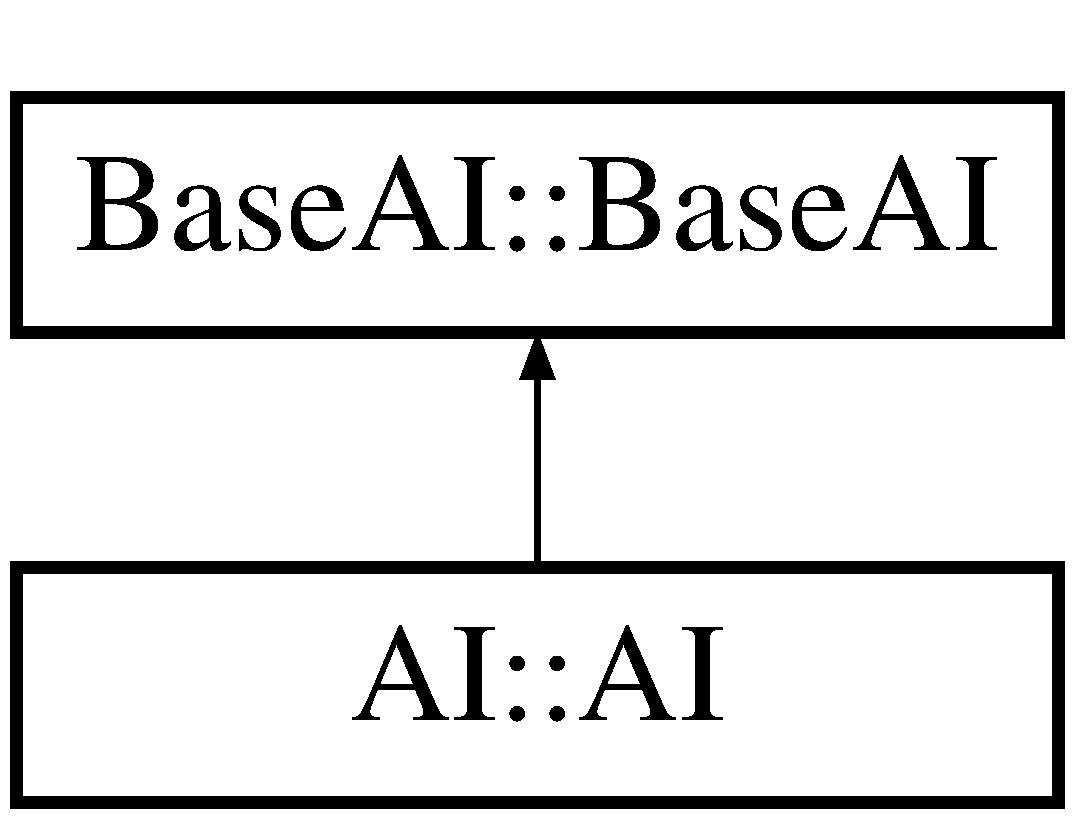
\includegraphics[height=2cm]{classAI_1_1AI}
\end{center}
\end{figure}
\subsection*{Public Member Functions}
\begin{DoxyCompactItemize}
\item 
\hypertarget{classAI_1_1AI_a1173d35565e571260327628b5fdbf601}{
def {\bfseries username}}
\label{classAI_1_1AI_a1173d35565e571260327628b5fdbf601}

\item 
\hypertarget{classAI_1_1AI_a0c68d55972c20f5b5c12b3413dccf4f8}{
def {\bfseries password}}
\label{classAI_1_1AI_a0c68d55972c20f5b5c12b3413dccf4f8}

\item 
\hypertarget{classAI_1_1AI_abe85fa052f61e71327d0f066866360ec}{
def {\bfseries init}}
\label{classAI_1_1AI_abe85fa052f61e71327d0f066866360ec}

\item 
\hypertarget{classAI_1_1AI_a0e95ce8db48896cbf1dcf410930ca141}{
def {\bfseries run}}
\label{classAI_1_1AI_a0e95ce8db48896cbf1dcf410930ca141}

\item 
\hypertarget{classAI_1_1AI_a98bd949e1d0d87db3c02a1453415f73e}{
def {\bfseries findAttackTarget}}
\label{classAI_1_1AI_a98bd949e1d0d87db3c02a1453415f73e}

\item 
\hypertarget{classAI_1_1AI_a0d332a883d380a3c4325d766eb66b911}{
def {\bfseries findMoveTarget}}
\label{classAI_1_1AI_a0d332a883d380a3c4325d766eb66b911}

\item 
\hypertarget{classAI_1_1AI_abd85a17fab96a0abe54bae971206824f}{
def {\bfseries moveOrKite}}
\label{classAI_1_1AI_abd85a17fab96a0abe54bae971206824f}

\item 
\hypertarget{classAI_1_1AI_a0d31a8b32480e4b425061ecf4c01f476}{
def {\bfseries collisionSafe}}
\label{classAI_1_1AI_a0d31a8b32480e4b425061ecf4c01f476}

\item 
\hypertarget{classAI_1_1AI_afc336c04d31701982b4aa115de277f2a}{
def {\bfseries \_\-\_\-init\_\-\_\-}}
\label{classAI_1_1AI_afc336c04d31701982b4aa115de277f2a}

\end{DoxyCompactItemize}
\subsection*{Public Attributes}
\begin{DoxyCompactItemize}
\item 
\hypertarget{classAI_1_1AI_aaef6cc5f313e3a1ec3e55b580fac14ca}{
{\bfseries stage}}
\label{classAI_1_1AI_aaef6cc5f313e3a1ec3e55b580fac14ca}

\end{DoxyCompactItemize}
\subsection*{Static Public Attributes}
\begin{DoxyCompactItemize}
\item 
\hypertarget{classAI_1_1AI_a7f63360325c448cc62d691c1705b7db1}{
int {\bfseries stage} = 0}
\label{classAI_1_1AI_a7f63360325c448cc62d691c1705b7db1}

\item 
\hypertarget{classAI_1_1AI_aaca1a89f8af8f3effe049e134b3b9fc6}{
int {\bfseries buildCoeff} = 8}
\label{classAI_1_1AI_aaca1a89f8af8f3effe049e134b3b9fc6}

\end{DoxyCompactItemize}


\subsection{Detailed Description}
\begin{DoxyVerb}The class implementing gameplay logic.\end{DoxyVerb}
 

The documentation for this class was generated from the following file:\begin{DoxyCompactItemize}
\item 
AI.py\end{DoxyCompactItemize}

\hypertarget{classBaseAI_1_1BaseAI}{
\section{BaseAI::BaseAI Class Reference}
\label{classBaseAI_1_1BaseAI}\index{BaseAI::BaseAI@{BaseAI::BaseAI}}
}
Inheritance diagram for BaseAI::BaseAI:\begin{figure}[H]
\begin{center}
\leavevmode
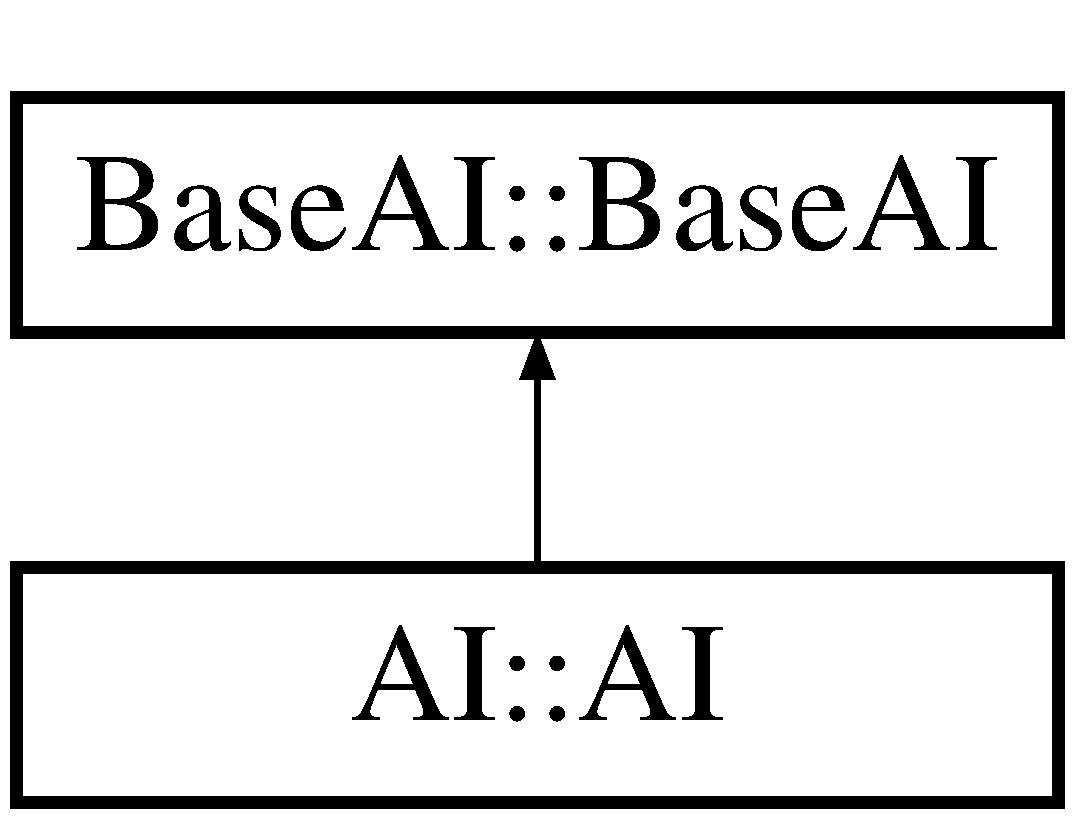
\includegraphics[height=2cm]{classBaseAI_1_1BaseAI}
\end{center}
\end{figure}
\subsection*{Public Member Functions}
\begin{DoxyCompactItemize}
\item 
\hypertarget{classBaseAI_1_1BaseAI_a2dcbc8732112a39869c75ed9f0771633}{
def {\bfseries startTurn}}
\label{classBaseAI_1_1BaseAI_a2dcbc8732112a39869c75ed9f0771633}

\item 
\hypertarget{classBaseAI_1_1BaseAI_afa3d3ad590dd453c4d064a3c16b7f1a8}{
def {\bfseries turnNumber}}
\label{classBaseAI_1_1BaseAI_afa3d3ad590dd453c4d064a3c16b7f1a8}

\item 
\hypertarget{classBaseAI_1_1BaseAI_a60e0d6b3832faae7c85b4c9f0be10196}{
def {\bfseries playerID}}
\label{classBaseAI_1_1BaseAI_a60e0d6b3832faae7c85b4c9f0be10196}

\item 
\hypertarget{classBaseAI_1_1BaseAI_ae83628dc59335aa5c77e96ffcd57ce92}{
def {\bfseries boardX}}
\label{classBaseAI_1_1BaseAI_ae83628dc59335aa5c77e96ffcd57ce92}

\item 
\hypertarget{classBaseAI_1_1BaseAI_a6148bb3c3c46a7b33ce1818fd41eb605}{
def {\bfseries boardY}}
\label{classBaseAI_1_1BaseAI_a6148bb3c3c46a7b33ce1818fd41eb605}

\item 
\hypertarget{classBaseAI_1_1BaseAI_a32416775fed0eb83efe7221d732cbd70}{
def {\bfseries gameNumber}}
\label{classBaseAI_1_1BaseAI_a32416775fed0eb83efe7221d732cbd70}

\item 
\hypertarget{classBaseAI_1_1BaseAI_a3bf925534912eaebc263179a9c058f17}{
def {\bfseries player0Time}}
\label{classBaseAI_1_1BaseAI_a3bf925534912eaebc263179a9c058f17}

\item 
\hypertarget{classBaseAI_1_1BaseAI_a947dcca2869c60f33dbb3b553d70a321}{
def {\bfseries player1Time}}
\label{classBaseAI_1_1BaseAI_a947dcca2869c60f33dbb3b553d70a321}

\item 
\hypertarget{classBaseAI_1_1BaseAI_a0b938d864530091b6efd420a2ed38d10}{
def {\bfseries \_\-\_\-init\_\-\_\-}}
\label{classBaseAI_1_1BaseAI_a0b938d864530091b6efd420a2ed38d10}

\end{DoxyCompactItemize}
\subsection*{Static Public Attributes}
\begin{DoxyCompactItemize}
\item 
\hypertarget{classBaseAI_1_1BaseAI_a32a836eb9aad27c111583f24238a686c}{
{\bfseries initialized} = False}
\label{classBaseAI_1_1BaseAI_a32a836eb9aad27c111583f24238a686c}

\item 
\hypertarget{classBaseAI_1_1BaseAI_a54d7182ce68d3d2b55d247c431561f9d}{
int {\bfseries iteration} = 0}
\label{classBaseAI_1_1BaseAI_a54d7182ce68d3d2b55d247c431561f9d}

\item 
\hypertarget{classBaseAI_1_1BaseAI_af78c73cdbcca5a8ed213e2510fbd6e94}{
{\bfseries runGenerator} = None}
\label{classBaseAI_1_1BaseAI_af78c73cdbcca5a8ed213e2510fbd6e94}

\item 
\hypertarget{classBaseAI_1_1BaseAI_a319a81bb1af508789e826e78ee727418}{
{\bfseries connection} = None}
\label{classBaseAI_1_1BaseAI_a319a81bb1af508789e826e78ee727418}

\item 
\hypertarget{classBaseAI_1_1BaseAI_aa6bab172dcc72b435a5fb3278d3d04e7}{
list {\bfseries bots} = \mbox{[}$\,$\mbox{]}}
\label{classBaseAI_1_1BaseAI_aa6bab172dcc72b435a5fb3278d3d04e7}

\item 
\hypertarget{classBaseAI_1_1BaseAI_a624a3b6f071e5d79a884bf87d036ed33}{
list {\bfseries frames} = \mbox{[}$\,$\mbox{]}}
\label{classBaseAI_1_1BaseAI_a624a3b6f071e5d79a884bf87d036ed33}

\item 
\hypertarget{classBaseAI_1_1BaseAI_a7d91c75817bc5a92c703225f5d65749b}{
list {\bfseries walls} = \mbox{[}$\,$\mbox{]}}
\label{classBaseAI_1_1BaseAI_a7d91c75817bc5a92c703225f5d65749b}

\item 
\hypertarget{classBaseAI_1_1BaseAI_a215884bd35440caa62fd5e9be088ac2f}{
list {\bfseries types} = \mbox{[}$\,$\mbox{]}}
\label{classBaseAI_1_1BaseAI_a215884bd35440caa62fd5e9be088ac2f}

\end{DoxyCompactItemize}


\subsection{Detailed Description}
\begin{DoxyVerb}@brief A basic AI interface.

This class implements most the code an AI would need to interface with the lower-level game code.
AIs should extend this class to get a lot of builer-plate code out of the way
The provided AI class does just that.
\end{DoxyVerb}
 

The documentation for this class was generated from the following file:\begin{DoxyCompactItemize}
\item 
BaseAI.py\end{DoxyCompactItemize}

\hypertarget{classGameObject_1_1Bot}{
\section{GameObject::Bot Class Reference}
\label{classGameObject_1_1Bot}\index{GameObject::Bot@{GameObject::Bot}}
}


The bot class.  


Inheritance diagram for GameObject::Bot:\begin{figure}[H]
\begin{center}
\leavevmode
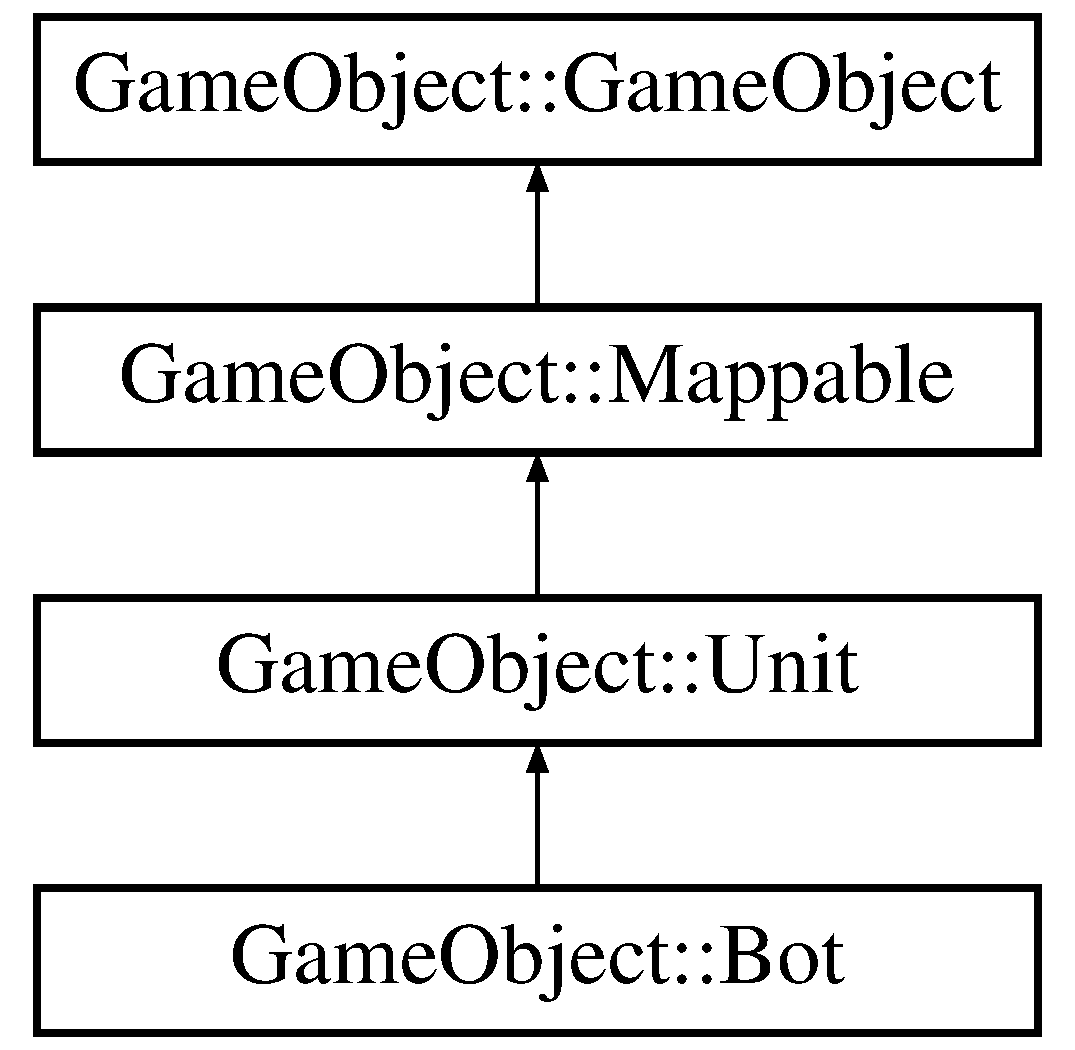
\includegraphics[height=4cm]{classGameObject_1_1Bot}
\end{center}
\end{figure}
\subsection*{Public Member Functions}
\begin{DoxyCompactItemize}
\item 
\hypertarget{classGameObject_1_1Bot_ae14fbf2780a8ee51c224f9fa2e841a27}{
def {\bfseries \_\-\_\-init\_\-\_\-}}
\label{classGameObject_1_1Bot_ae14fbf2780a8ee51c224f9fa2e841a27}

\item 
\hypertarget{classGameObject_1_1Bot_a519b951174aa9a7c58cf41e5ba4c237d}{
def {\bfseries validify}}
\label{classGameObject_1_1Bot_a519b951174aa9a7c58cf41e5ba4c237d}

\item 
\hypertarget{classGameObject_1_1Bot_ab6f7a4db8f18482b6016ce4fd42978ad}{
def \hyperlink{classGameObject_1_1Bot_ab6f7a4db8f18482b6016ce4fd42978ad}{talk}}
\label{classGameObject_1_1Bot_ab6f7a4db8f18482b6016ce4fd42978ad}

\begin{DoxyCompactList}\small\item\em Sends a message to be visualized when this unit is selected. \item\end{DoxyCompactList}\item 
def \hyperlink{classGameObject_1_1Bot_a1a55ec801c2aff9eee777579972ad6ef}{move}
\begin{DoxyCompactList}\small\item\em Move in the indicated direction (U, D, L, or R). \item\end{DoxyCompactList}\item 
def \hyperlink{classGameObject_1_1Bot_a20ce42e67cc1586a7086b708c56b6609}{attack}
\begin{DoxyCompactList}\small\item\em Attack the specified unit. \item\end{DoxyCompactList}\item 
def \hyperlink{classGameObject_1_1Bot_ab0d8899c1214ba9b4311300dc0e7cb1b}{heal}
\begin{DoxyCompactList}\small\item\em Heals the indicated bot. \item\end{DoxyCompactList}\item 
def \hyperlink{classGameObject_1_1Bot_acb307f9ba536de899c113047d2599d05}{build}
\begin{DoxyCompactList}\small\item\em Begins building a new robot. \item\end{DoxyCompactList}\item 
def \hyperlink{classGameObject_1_1Bot_a86ef5a544c38e3bcbfc961ab5d4ff58f}{combine}
\begin{DoxyCompactList}\small\item\em Combines four robots into one. \item\end{DoxyCompactList}\item 
def \hyperlink{classGameObject_1_1Bot_a580aa8beb8bf56bbd471db9474865b11}{split}
\begin{DoxyCompactList}\small\item\em Splits a compound bot into the 4 robots that combined to make it. \item\end{DoxyCompactList}\item 
def \hyperlink{classGameObject_1_1Bot_ac926e9da58f96ee5996d22e609d1a41e}{maxActions}
\begin{DoxyCompactList}\small\item\em Returns the maximum number of actions this robot can take per turn. \item\end{DoxyCompactList}\item 
def \hyperlink{classGameObject_1_1Bot_ab2f7439ed0465837575635fadcd04e48}{maxSteps}
\begin{DoxyCompactList}\small\item\em Returns the maximum number of steps this robot can take per turn. \item\end{DoxyCompactList}\item 
\hypertarget{classGameObject_1_1Bot_ae315ea2bbf2580ad9472142793e33603}{
def \hyperlink{classGameObject_1_1Bot_ae315ea2bbf2580ad9472142793e33603}{getId}}
\label{classGameObject_1_1Bot_ae315ea2bbf2580ad9472142793e33603}

\begin{DoxyCompactList}\small\item\em Unique Identifier. \item\end{DoxyCompactList}\item 
def \hyperlink{classGameObject_1_1Bot_a76521d97d7dcce093efbdd1926c75750}{getX}
\begin{DoxyCompactList}\small\item\em The X position of the top left corner of this object. \item\end{DoxyCompactList}\item 
def \hyperlink{classGameObject_1_1Bot_a5e193704cae24529a6e6f00fd9a1447f}{getY}
\begin{DoxyCompactList}\small\item\em The Y position of the top left corner of this object. \item\end{DoxyCompactList}\item 
\hypertarget{classGameObject_1_1Bot_aac97597e773e01e0bc9097b72348da29}{
def \hyperlink{classGameObject_1_1Bot_aac97597e773e01e0bc9097b72348da29}{getOwner}}
\label{classGameObject_1_1Bot_aac97597e773e01e0bc9097b72348da29}

\begin{DoxyCompactList}\small\item\em The owning player. \item\end{DoxyCompactList}\item 
\hypertarget{classGameObject_1_1Bot_a3009ec43cd1c14fd1bc1c3acd278d8a0}{
def \hyperlink{classGameObject_1_1Bot_a3009ec43cd1c14fd1bc1c3acd278d8a0}{getHealth}}
\label{classGameObject_1_1Bot_a3009ec43cd1c14fd1bc1c3acd278d8a0}

\begin{DoxyCompactList}\small\item\em How much health this unit currently has. \item\end{DoxyCompactList}\item 
\hypertarget{classGameObject_1_1Bot_aae97e27e3951b3e7149378fa7ca8a74b}{
def \hyperlink{classGameObject_1_1Bot_aae97e27e3951b3e7149378fa7ca8a74b}{getMaxHealth}}
\label{classGameObject_1_1Bot_aae97e27e3951b3e7149378fa7ca8a74b}

\begin{DoxyCompactList}\small\item\em The maximum amount of health this unit can ever have. \item\end{DoxyCompactList}\item 
\hypertarget{classGameObject_1_1Bot_a4ff82e790545eae1767ce5ef581213e8}{
def \hyperlink{classGameObject_1_1Bot_a4ff82e790545eae1767ce5ef581213e8}{getSize}}
\label{classGameObject_1_1Bot_a4ff82e790545eae1767ce5ef581213e8}

\begin{DoxyCompactList}\small\item\em The length of one side of this \hyperlink{classGameObject_1_1Unit}{Unit}. \item\end{DoxyCompactList}\item 
\hypertarget{classGameObject_1_1Bot_ab65146e76f34066858a00e29a01d8aac}{
def \hyperlink{classGameObject_1_1Bot_ab65146e76f34066858a00e29a01d8aac}{getActions}}
\label{classGameObject_1_1Bot_ab65146e76f34066858a00e29a01d8aac}

\begin{DoxyCompactList}\small\item\em How many actions this bot can still perform. \item\end{DoxyCompactList}\item 
\hypertarget{classGameObject_1_1Bot_a9abaae7ee4a01ff06d13803eaf0ebc72}{
def \hyperlink{classGameObject_1_1Bot_a9abaae7ee4a01ff06d13803eaf0ebc72}{getSteps}}
\label{classGameObject_1_1Bot_a9abaae7ee4a01ff06d13803eaf0ebc72}

\begin{DoxyCompactList}\small\item\em How many steps this bot can still take. \item\end{DoxyCompactList}\item 
\hypertarget{classGameObject_1_1Bot_a30aa5cc047d6441579158e76d63896d9}{
def \hyperlink{classGameObject_1_1Bot_a30aa5cc047d6441579158e76d63896d9}{getDamage}}
\label{classGameObject_1_1Bot_a30aa5cc047d6441579158e76d63896d9}

\begin{DoxyCompactList}\small\item\em The amount of damage this robot does when attacking. \item\end{DoxyCompactList}\item 
\hypertarget{classGameObject_1_1Bot_a6892f5fd85e000e6052c4073f6fb1398}{
def \hyperlink{classGameObject_1_1Bot_a6892f5fd85e000e6052c4073f6fb1398}{getRange}}
\label{classGameObject_1_1Bot_a6892f5fd85e000e6052c4073f6fb1398}

\begin{DoxyCompactList}\small\item\em How far this robot can attack or heal from its edge. \item\end{DoxyCompactList}\item 
\hypertarget{classGameObject_1_1Bot_aa5ecd238c3fdf1b123dc9e5c2e634121}{
def \hyperlink{classGameObject_1_1Bot_aa5ecd238c3fdf1b123dc9e5c2e634121}{getMovitude}}
\label{classGameObject_1_1Bot_aa5ecd238c3fdf1b123dc9e5c2e634121}

\begin{DoxyCompactList}\small\item\em This value divided by the number of bots = maxSteps for this robot. \item\end{DoxyCompactList}\item 
\hypertarget{classGameObject_1_1Bot_a810470c6f1aeaad5880ac126ca6a532c}{
def \hyperlink{classGameObject_1_1Bot_a810470c6f1aeaad5880ac126ca6a532c}{getActitude}}
\label{classGameObject_1_1Bot_a810470c6f1aeaad5880ac126ca6a532c}

\begin{DoxyCompactList}\small\item\em This value divided by the number of bots = maxActions for this robot. \item\end{DoxyCompactList}\item 
\hypertarget{classGameObject_1_1Bot_a78f4bdba8edf04f46bbe9e02041ce6a1}{
def \hyperlink{classGameObject_1_1Bot_a78f4bdba8edf04f46bbe9e02041ce6a1}{getBuildRate}}
\label{classGameObject_1_1Bot_a78f4bdba8edf04f46bbe9e02041ce6a1}

\begin{DoxyCompactList}\small\item\em This value is used to determine how many turns it takes to build a robot and how much this robot heals for. \item\end{DoxyCompactList}\item 
\hypertarget{classGameObject_1_1Bot_a74143a60984b638ceebccb84056e6474}{
def \hyperlink{classGameObject_1_1Bot_a74143a60984b638ceebccb84056e6474}{getPartOf}}
\label{classGameObject_1_1Bot_a74143a60984b638ceebccb84056e6474}

\begin{DoxyCompactList}\small\item\em ID of the robot this robot is apart of, 0 if not in a robot. \item\end{DoxyCompactList}\item 
\hypertarget{classGameObject_1_1Bot_a8629a4748225228f6b6d65fb3a9982d6}{
def \hyperlink{classGameObject_1_1Bot_a8629a4748225228f6b6d65fb3a9982d6}{getBuilding}}
\label{classGameObject_1_1Bot_a8629a4748225228f6b6d65fb3a9982d6}

\begin{DoxyCompactList}\small\item\em ID of the robot this robot is building, 0 if not building. \item\end{DoxyCompactList}\item 
\hypertarget{classGameObject_1_1Bot_a98e2b4a8d933ec347826c89b57304b6e}{
def \hyperlink{classGameObject_1_1Bot_a98e2b4a8d933ec347826c89b57304b6e}{getType}}
\label{classGameObject_1_1Bot_a98e2b4a8d933ec347826c89b57304b6e}

\begin{DoxyCompactList}\small\item\em ID of the type this robot is, 0 if a combination. \item\end{DoxyCompactList}\item 
\hypertarget{classGameObject_1_1Bot_a9d9b75c68d6ccef5fbabc407cacbc9f5}{
def {\bfseries \_\-\_\-str\_\-\_\-}}
\label{classGameObject_1_1Bot_a9d9b75c68d6ccef5fbabc407cacbc9f5}

\end{DoxyCompactItemize}
\subsection*{Public Attributes}
\begin{DoxyCompactItemize}
\item 
\hypertarget{classGameObject_1_1Bot_afc115a9af2389b809a3e33aa3deb31dd}{
{\bfseries ptr}}
\label{classGameObject_1_1Bot_afc115a9af2389b809a3e33aa3deb31dd}

\item 
\hypertarget{classGameObject_1_1Bot_a299e4ce1e2b005f955ce4b8032e1e1c4}{
{\bfseries iteration}}
\label{classGameObject_1_1Bot_a299e4ce1e2b005f955ce4b8032e1e1c4}

\item 
\hypertarget{classGameObject_1_1Bot_a964267f61141849cd7eea884de9d5259}{
{\bfseries id}}
\label{classGameObject_1_1Bot_a964267f61141849cd7eea884de9d5259}

\end{DoxyCompactItemize}


\subsection{Detailed Description}
The bot class. 

\subsection{Member Function Documentation}
\hypertarget{classGameObject_1_1Bot_a20ce42e67cc1586a7086b708c56b6609}{
\index{GameObject::Bot@{GameObject::Bot}!attack@{attack}}
\index{attack@{attack}!GameObject::Bot@{GameObject::Bot}}
\subsubsection[{attack}]{\setlength{\rightskip}{0pt plus 5cm}def GameObject::Bot::attack ( {\em self}, \/   {\em target})}}
\label{classGameObject_1_1Bot_a20ce42e67cc1586a7086b708c56b6609}


Attack the specified unit. 

Requires the calling robot to have an action and for the target to be in range \hypertarget{classGameObject_1_1Bot_acb307f9ba536de899c113047d2599d05}{
\index{GameObject::Bot@{GameObject::Bot}!build@{build}}
\index{build@{build}!GameObject::Bot@{GameObject::Bot}}
\subsubsection[{build}]{\setlength{\rightskip}{0pt plus 5cm}def GameObject::Bot::build ( {\em self}, \/   {\em type}, \/   {\em x}, \/   {\em y}, \/   {\em size})}}
\label{classGameObject_1_1Bot_acb307f9ba536de899c113047d2599d05}


Begins building a new robot. 

While building, the new robot will be a frame. Requires the calling robot to have an action. X and Y must cause the new robot to be adjacent. Size must be less than or equal to the calling robots size. Completes in 8 $\ast$ size$^\wedge$2 / self.buildRate turns \hypertarget{classGameObject_1_1Bot_a86ef5a544c38e3bcbfc961ab5d4ff58f}{
\index{GameObject::Bot@{GameObject::Bot}!combine@{combine}}
\index{combine@{combine}!GameObject::Bot@{GameObject::Bot}}
\subsubsection[{combine}]{\setlength{\rightskip}{0pt plus 5cm}def GameObject::Bot::combine ( {\em self}, \/   {\em bot2}, \/   {\em bot3}, \/   {\em bot4})}}
\label{classGameObject_1_1Bot_a86ef5a544c38e3bcbfc961ab5d4ff58f}


Combines four robots into one. 

Requires all robots to have an action, be of the same size, and be arranged in a square \hypertarget{classGameObject_1_1Bot_a76521d97d7dcce093efbdd1926c75750}{
\index{GameObject::Bot@{GameObject::Bot}!getX@{getX}}
\index{getX@{getX}!GameObject::Bot@{GameObject::Bot}}
\subsubsection[{getX}]{\setlength{\rightskip}{0pt plus 5cm}def GameObject::Bot::getX ( {\em self})}}
\label{classGameObject_1_1Bot_a76521d97d7dcce093efbdd1926c75750}


The X position of the top left corner of this object. 

X is horizontal 

Reimplemented from \hyperlink{classGameObject_1_1Unit_a01711efd87c7e3e2a97066e9a5c50da5}{GameObject::Unit}.

\hypertarget{classGameObject_1_1Bot_a5e193704cae24529a6e6f00fd9a1447f}{
\index{GameObject::Bot@{GameObject::Bot}!getY@{getY}}
\index{getY@{getY}!GameObject::Bot@{GameObject::Bot}}
\subsubsection[{getY}]{\setlength{\rightskip}{0pt plus 5cm}def GameObject::Bot::getY ( {\em self})}}
\label{classGameObject_1_1Bot_a5e193704cae24529a6e6f00fd9a1447f}


The Y position of the top left corner of this object. 

Y is vertical 

Reimplemented from \hyperlink{classGameObject_1_1Unit_a4d0c47deb0ddb19b9e2b195d8ca2f2ad}{GameObject::Unit}.

\hypertarget{classGameObject_1_1Bot_ab0d8899c1214ba9b4311300dc0e7cb1b}{
\index{GameObject::Bot@{GameObject::Bot}!heal@{heal}}
\index{heal@{heal}!GameObject::Bot@{GameObject::Bot}}
\subsubsection[{heal}]{\setlength{\rightskip}{0pt plus 5cm}def GameObject::Bot::heal ( {\em self}, \/   {\em target})}}
\label{classGameObject_1_1Bot_ab0d8899c1214ba9b4311300dc0e7cb1b}


Heals the indicated bot. 

Requires the calling robot to have an action and for the target to be in range. Heals for target.maxHealth $\ast$ self.buildRate / (4 $\ast$ target.size$^\wedge$2) \hypertarget{classGameObject_1_1Bot_ac926e9da58f96ee5996d22e609d1a41e}{
\index{GameObject::Bot@{GameObject::Bot}!maxActions@{maxActions}}
\index{maxActions@{maxActions}!GameObject::Bot@{GameObject::Bot}}
\subsubsection[{maxActions}]{\setlength{\rightskip}{0pt plus 5cm}def GameObject::Bot::maxActions ( {\em self})}}
\label{classGameObject_1_1Bot_ac926e9da58f96ee5996d22e609d1a41e}


Returns the maximum number of actions this robot can take per turn. 

\hypertarget{classGameObject_1_1Bot_ab2f7439ed0465837575635fadcd04e48}{
\index{GameObject::Bot@{GameObject::Bot}!maxSteps@{maxSteps}}
\index{maxSteps@{maxSteps}!GameObject::Bot@{GameObject::Bot}}
\subsubsection[{maxSteps}]{\setlength{\rightskip}{0pt plus 5cm}def GameObject::Bot::maxSteps ( {\em self})}}
\label{classGameObject_1_1Bot_ab2f7439ed0465837575635fadcd04e48}


Returns the maximum number of steps this robot can take per turn. 

\hypertarget{classGameObject_1_1Bot_a1a55ec801c2aff9eee777579972ad6ef}{
\index{GameObject::Bot@{GameObject::Bot}!move@{move}}
\index{move@{move}!GameObject::Bot@{GameObject::Bot}}
\subsubsection[{move}]{\setlength{\rightskip}{0pt plus 5cm}def GameObject::Bot::move ( {\em self}, \/   {\em direction})}}
\label{classGameObject_1_1Bot_a1a55ec801c2aff9eee777579972ad6ef}


Move in the indicated direction (U, D, L, or R). 

U is y=y-\/1, L=x=x-\/1, such that the top left corner is (0,0). Requires the calling robot to have a step. \hypertarget{classGameObject_1_1Bot_a580aa8beb8bf56bbd471db9474865b11}{
\index{GameObject::Bot@{GameObject::Bot}!split@{split}}
\index{split@{split}!GameObject::Bot@{GameObject::Bot}}
\subsubsection[{split}]{\setlength{\rightskip}{0pt plus 5cm}def GameObject::Bot::split ( {\em self})}}
\label{classGameObject_1_1Bot_a580aa8beb8bf56bbd471db9474865b11}


Splits a compound bot into the 4 robots that combined to make it. 

Requires the calling robot to have an action. 

The documentation for this class was generated from the following file:\begin{DoxyCompactItemize}
\item 
GameObject.py\end{DoxyCompactItemize}

\hypertarget{classExistentialError_1_1ExistentialError}{
\section{ExistentialError::ExistentialError Class Reference}
\label{classExistentialError_1_1ExistentialError}\index{ExistentialError::ExistentialError@{ExistentialError::ExistentialError}}
}


The documentation for this class was generated from the following file:\begin{DoxyCompactItemize}
\item 
ExistentialError.py\end{DoxyCompactItemize}

\hypertarget{classGameObject_1_1Frame}{
\section{GameObject::Frame Class Reference}
\label{classGameObject_1_1Frame}\index{GameObject::Frame@{GameObject::Frame}}
}


A baby robot.  


Inheritance diagram for GameObject::Frame:\begin{figure}[H]
\begin{center}
\leavevmode
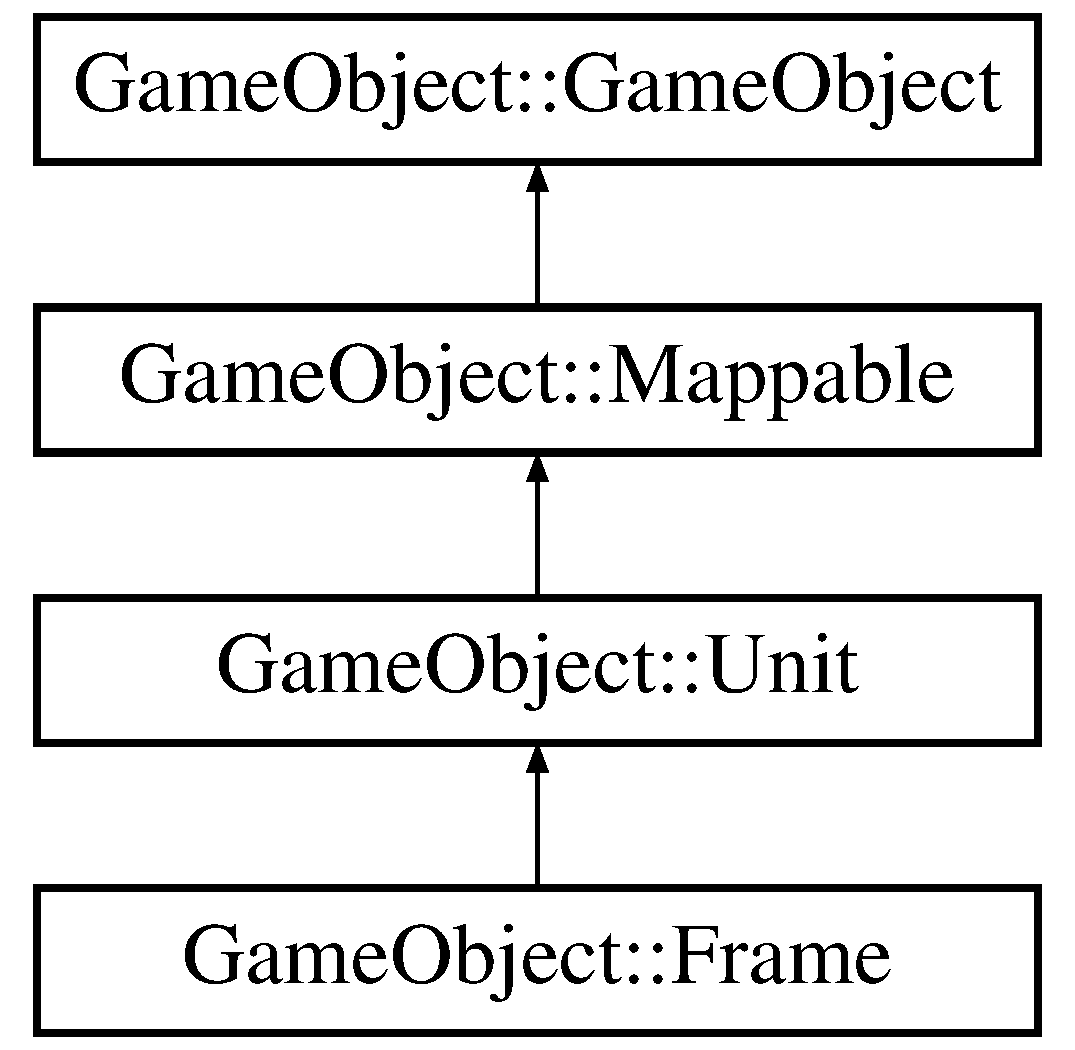
\includegraphics[height=4cm]{classGameObject_1_1Frame}
\end{center}
\end{figure}
\subsection*{Public Member Functions}
\begin{DoxyCompactItemize}
\item 
\hypertarget{classGameObject_1_1Frame_a0c7f646fd6d560f543c2e4a42879c746}{
def {\bfseries \_\-\_\-init\_\-\_\-}}
\label{classGameObject_1_1Frame_a0c7f646fd6d560f543c2e4a42879c746}

\item 
\hypertarget{classGameObject_1_1Frame_a3b3469de753098bee40ab13079c0b6ec}{
def {\bfseries validify}}
\label{classGameObject_1_1Frame_a3b3469de753098bee40ab13079c0b6ec}

\item 
\hypertarget{classGameObject_1_1Frame_af6a8745cc68bb4bd36c2f370c1041e93}{
def \hyperlink{classGameObject_1_1Frame_af6a8745cc68bb4bd36c2f370c1041e93}{talk}}
\label{classGameObject_1_1Frame_af6a8745cc68bb4bd36c2f370c1041e93}

\begin{DoxyCompactList}\small\item\em Sends a message to be visualized when this unit is selected. \item\end{DoxyCompactList}\item 
\hypertarget{classGameObject_1_1Frame_a2f554cee1f85539ad4b656a91f1aaf07}{
def \hyperlink{classGameObject_1_1Frame_a2f554cee1f85539ad4b656a91f1aaf07}{getId}}
\label{classGameObject_1_1Frame_a2f554cee1f85539ad4b656a91f1aaf07}

\begin{DoxyCompactList}\small\item\em Unique Identifier. \item\end{DoxyCompactList}\item 
def \hyperlink{classGameObject_1_1Frame_aab513e4859fc8a9f5d5f1a6b47cb6df3}{getX}
\begin{DoxyCompactList}\small\item\em The X position of the top left corner of this object. \item\end{DoxyCompactList}\item 
def \hyperlink{classGameObject_1_1Frame_abf564d6f986b8e9d2a83838691c591f9}{getY}
\begin{DoxyCompactList}\small\item\em The Y position of the top left corner of this object. \item\end{DoxyCompactList}\item 
\hypertarget{classGameObject_1_1Frame_a2b57ecf997ea4cbedfae9cddf4f60fc7}{
def \hyperlink{classGameObject_1_1Frame_a2b57ecf997ea4cbedfae9cddf4f60fc7}{getOwner}}
\label{classGameObject_1_1Frame_a2b57ecf997ea4cbedfae9cddf4f60fc7}

\begin{DoxyCompactList}\small\item\em The owning player. \item\end{DoxyCompactList}\item 
\hypertarget{classGameObject_1_1Frame_af036b32ae2bcf9f4acd11fda90146de0}{
def \hyperlink{classGameObject_1_1Frame_af036b32ae2bcf9f4acd11fda90146de0}{getHealth}}
\label{classGameObject_1_1Frame_af036b32ae2bcf9f4acd11fda90146de0}

\begin{DoxyCompactList}\small\item\em How much health this unit currently has. \item\end{DoxyCompactList}\item 
\hypertarget{classGameObject_1_1Frame_a2a99efc2530cccc2df244e5afbdd2048}{
def \hyperlink{classGameObject_1_1Frame_a2a99efc2530cccc2df244e5afbdd2048}{getMaxHealth}}
\label{classGameObject_1_1Frame_a2a99efc2530cccc2df244e5afbdd2048}

\begin{DoxyCompactList}\small\item\em The maximum amount of health this unit can ever have. \item\end{DoxyCompactList}\item 
\hypertarget{classGameObject_1_1Frame_a472830a60e54160e0e0c745767f1003b}{
def \hyperlink{classGameObject_1_1Frame_a472830a60e54160e0e0c745767f1003b}{getSize}}
\label{classGameObject_1_1Frame_a472830a60e54160e0e0c745767f1003b}

\begin{DoxyCompactList}\small\item\em The length of one side of this \hyperlink{classGameObject_1_1Unit}{Unit}. \item\end{DoxyCompactList}\item 
\hypertarget{classGameObject_1_1Frame_a4ef8a1df648fef94d8eafcdb9402b600}{
def \hyperlink{classGameObject_1_1Frame_a4ef8a1df648fef94d8eafcdb9402b600}{getType}}
\label{classGameObject_1_1Frame_a4ef8a1df648fef94d8eafcdb9402b600}

\begin{DoxyCompactList}\small\item\em What type this robot will be. \item\end{DoxyCompactList}\item 
\hypertarget{classGameObject_1_1Frame_a01209c50114ad06ca2851d0aefeca33d}{
def \hyperlink{classGameObject_1_1Frame_a01209c50114ad06ca2851d0aefeca33d}{getCompletionTime}}
\label{classGameObject_1_1Frame_a01209c50114ad06ca2851d0aefeca33d}

\begin{DoxyCompactList}\small\item\em How many of your turns until this frame becomes a robot. \item\end{DoxyCompactList}\item 
\hypertarget{classGameObject_1_1Frame_aa6ad405de5401e9693cd83f83cc914e0}{
def {\bfseries \_\-\_\-str\_\-\_\-}}
\label{classGameObject_1_1Frame_aa6ad405de5401e9693cd83f83cc914e0}

\end{DoxyCompactItemize}
\subsection*{Public Attributes}
\begin{DoxyCompactItemize}
\item 
\hypertarget{classGameObject_1_1Frame_a8f947810e6ff714e270340b2927a2146}{
{\bfseries ptr}}
\label{classGameObject_1_1Frame_a8f947810e6ff714e270340b2927a2146}

\item 
\hypertarget{classGameObject_1_1Frame_a5e1552bc29afc173297363fb4825d018}{
{\bfseries iteration}}
\label{classGameObject_1_1Frame_a5e1552bc29afc173297363fb4825d018}

\item 
\hypertarget{classGameObject_1_1Frame_a920b0de70d007f5f6cd5a1a71c7741cb}{
{\bfseries id}}
\label{classGameObject_1_1Frame_a920b0de70d007f5f6cd5a1a71c7741cb}

\end{DoxyCompactItemize}


\subsection{Detailed Description}
A baby robot. 

\subsection{Member Function Documentation}
\hypertarget{classGameObject_1_1Frame_aab513e4859fc8a9f5d5f1a6b47cb6df3}{
\index{GameObject::Frame@{GameObject::Frame}!getX@{getX}}
\index{getX@{getX}!GameObject::Frame@{GameObject::Frame}}
\subsubsection[{getX}]{\setlength{\rightskip}{0pt plus 5cm}def GameObject::Frame::getX ( {\em self})}}
\label{classGameObject_1_1Frame_aab513e4859fc8a9f5d5f1a6b47cb6df3}


The X position of the top left corner of this object. 

X is horizontal 

Reimplemented from \hyperlink{classGameObject_1_1Unit_a01711efd87c7e3e2a97066e9a5c50da5}{GameObject::Unit}.

\hypertarget{classGameObject_1_1Frame_abf564d6f986b8e9d2a83838691c591f9}{
\index{GameObject::Frame@{GameObject::Frame}!getY@{getY}}
\index{getY@{getY}!GameObject::Frame@{GameObject::Frame}}
\subsubsection[{getY}]{\setlength{\rightskip}{0pt plus 5cm}def GameObject::Frame::getY ( {\em self})}}
\label{classGameObject_1_1Frame_abf564d6f986b8e9d2a83838691c591f9}


The Y position of the top left corner of this object. 

Y is vertical 

Reimplemented from \hyperlink{classGameObject_1_1Unit_a4d0c47deb0ddb19b9e2b195d8ca2f2ad}{GameObject::Unit}.



The documentation for this class was generated from the following file:\begin{DoxyCompactItemize}
\item 
GameObject.py\end{DoxyCompactItemize}

\hypertarget{classGameObject_1_1GameObject}{
\section{GameObject::GameObject Class Reference}
\label{classGameObject_1_1GameObject}\index{GameObject::GameObject@{GameObject::GameObject}}
}
Inheritance diagram for GameObject::GameObject:\begin{figure}[H]
\begin{center}
\leavevmode
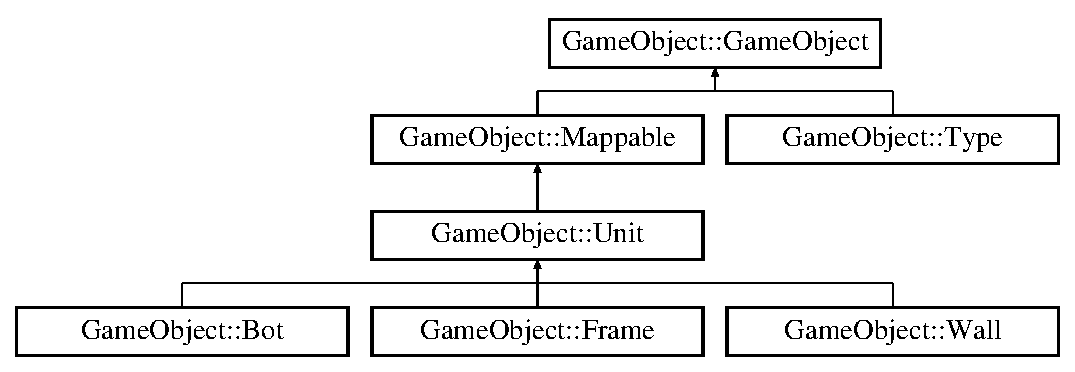
\includegraphics[height=4cm]{classGameObject_1_1GameObject}
\end{center}
\end{figure}
\subsection*{Public Member Functions}
\begin{DoxyCompactItemize}
\item 
\hypertarget{classGameObject_1_1GameObject_ab8fc51fb12907dfeb24e3396eff13252}{
def {\bfseries \_\-\_\-init\_\-\_\-}}
\label{classGameObject_1_1GameObject_ab8fc51fb12907dfeb24e3396eff13252}

\end{DoxyCompactItemize}
\subsection*{Public Attributes}
\begin{DoxyCompactItemize}
\item 
\hypertarget{classGameObject_1_1GameObject_ab09e368639157c6fa81535684ad600db}{
{\bfseries ptr}}
\label{classGameObject_1_1GameObject_ab09e368639157c6fa81535684ad600db}

\item 
\hypertarget{classGameObject_1_1GameObject_a36654bebef12ac56a2abf4988bb49c95}{
{\bfseries iteration}}
\label{classGameObject_1_1GameObject_a36654bebef12ac56a2abf4988bb49c95}

\end{DoxyCompactItemize}


The documentation for this class was generated from the following file:\begin{DoxyCompactItemize}
\item 
GameObject.py\end{DoxyCompactItemize}

\hypertarget{classGameObject_1_1Mappable}{
\section{GameObject::Mappable Class Reference}
\label{classGameObject_1_1Mappable}\index{GameObject::Mappable@{GameObject::Mappable}}
}


An object that exists on the grid.  


Inheritance diagram for GameObject::Mappable:\begin{figure}[H]
\begin{center}
\leavevmode
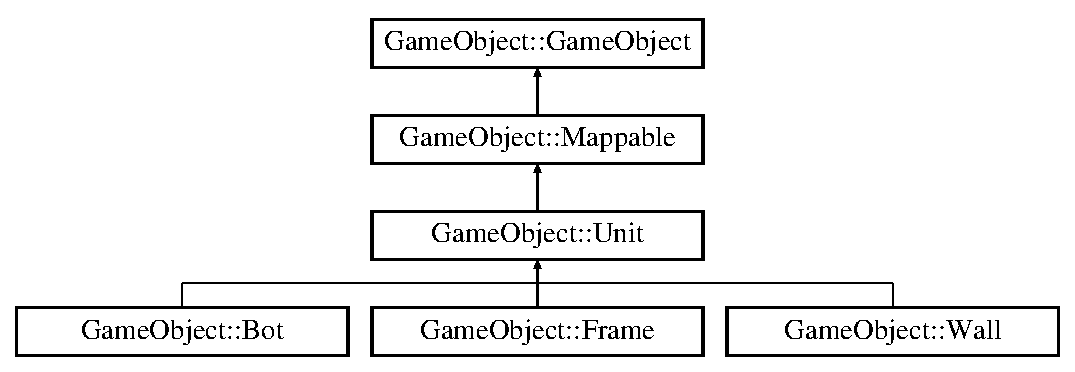
\includegraphics[height=4cm]{classGameObject_1_1Mappable}
\end{center}
\end{figure}
\subsection*{Public Member Functions}
\begin{DoxyCompactItemize}
\item 
\hypertarget{classGameObject_1_1Mappable_a3b50a330f5d310394f13a2514e0f5ee5}{
def {\bfseries \_\-\_\-init\_\-\_\-}}
\label{classGameObject_1_1Mappable_a3b50a330f5d310394f13a2514e0f5ee5}

\item 
\hypertarget{classGameObject_1_1Mappable_ac2b76487a93e9e56615dc47b4dcb0928}{
def \hyperlink{classGameObject_1_1Mappable_ac2b76487a93e9e56615dc47b4dcb0928}{getId}}
\label{classGameObject_1_1Mappable_ac2b76487a93e9e56615dc47b4dcb0928}

\begin{DoxyCompactList}\small\item\em Unique Identifier. \item\end{DoxyCompactList}\item 
def \hyperlink{classGameObject_1_1Mappable_a3ae7d302c87c0a6f1e211a7584c3b807}{getX}
\begin{DoxyCompactList}\small\item\em The X position of the top left corner of this object. \item\end{DoxyCompactList}\item 
def \hyperlink{classGameObject_1_1Mappable_af7b558a1be2dc80d1aa78f306e226c10}{getY}
\begin{DoxyCompactList}\small\item\em The Y position of the top left corner of this object. \item\end{DoxyCompactList}\item 
\hypertarget{classGameObject_1_1Mappable_ac999580cd8c2dad4d0f6200875bdb0f7}{
def {\bfseries \_\-\_\-str\_\-\_\-}}
\label{classGameObject_1_1Mappable_ac999580cd8c2dad4d0f6200875bdb0f7}

\end{DoxyCompactItemize}
\subsection*{Public Attributes}
\begin{DoxyCompactItemize}
\item 
\hypertarget{classGameObject_1_1Mappable_a062d225b787ddf7fc28a3ca50d1e1d2d}{
{\bfseries ptr}}
\label{classGameObject_1_1Mappable_a062d225b787ddf7fc28a3ca50d1e1d2d}

\item 
\hypertarget{classGameObject_1_1Mappable_a21e112d15966584c1e4f165de52a4ef5}{
{\bfseries iteration}}
\label{classGameObject_1_1Mappable_a21e112d15966584c1e4f165de52a4ef5}

\item 
\hypertarget{classGameObject_1_1Mappable_a952b8d62ae9d11a73fa1b2ec2c0244b6}{
{\bfseries id}}
\label{classGameObject_1_1Mappable_a952b8d62ae9d11a73fa1b2ec2c0244b6}

\end{DoxyCompactItemize}


\subsection{Detailed Description}
An object that exists on the grid. 

\subsection{Member Function Documentation}
\hypertarget{classGameObject_1_1Mappable_a3ae7d302c87c0a6f1e211a7584c3b807}{
\index{GameObject::Mappable@{GameObject::Mappable}!getX@{getX}}
\index{getX@{getX}!GameObject::Mappable@{GameObject::Mappable}}
\subsubsection[{getX}]{\setlength{\rightskip}{0pt plus 5cm}def GameObject::Mappable::getX ( {\em self})}}
\label{classGameObject_1_1Mappable_a3ae7d302c87c0a6f1e211a7584c3b807}


The X position of the top left corner of this object. 

X is horizontal 

Reimplemented in \hyperlink{classGameObject_1_1Unit_a01711efd87c7e3e2a97066e9a5c50da5}{GameObject::Unit}, \hyperlink{classGameObject_1_1Bot_a76521d97d7dcce093efbdd1926c75750}{GameObject::Bot}, \hyperlink{classGameObject_1_1Frame_aab513e4859fc8a9f5d5f1a6b47cb6df3}{GameObject::Frame}, and \hyperlink{classGameObject_1_1Wall_aa8d092fd75ef8372aacf4ece64521ea8}{GameObject::Wall}.

\hypertarget{classGameObject_1_1Mappable_af7b558a1be2dc80d1aa78f306e226c10}{
\index{GameObject::Mappable@{GameObject::Mappable}!getY@{getY}}
\index{getY@{getY}!GameObject::Mappable@{GameObject::Mappable}}
\subsubsection[{getY}]{\setlength{\rightskip}{0pt plus 5cm}def GameObject::Mappable::getY ( {\em self})}}
\label{classGameObject_1_1Mappable_af7b558a1be2dc80d1aa78f306e226c10}


The Y position of the top left corner of this object. 

Y is vertical 

Reimplemented in \hyperlink{classGameObject_1_1Unit_a4d0c47deb0ddb19b9e2b195d8ca2f2ad}{GameObject::Unit}, \hyperlink{classGameObject_1_1Bot_a5e193704cae24529a6e6f00fd9a1447f}{GameObject::Bot}, \hyperlink{classGameObject_1_1Frame_abf564d6f986b8e9d2a83838691c591f9}{GameObject::Frame}, and \hyperlink{classGameObject_1_1Wall_ac87b620714dfacc5ac12ca6078a91460}{GameObject::Wall}.



The documentation for this class was generated from the following file:\begin{DoxyCompactItemize}
\item 
GameObject.py\end{DoxyCompactItemize}

\hypertarget{classGameObject_1_1Type}{
\section{GameObject::Type Class Reference}
\label{classGameObject_1_1Type}\index{GameObject::Type@{GameObject::Type}}
}


A kind of robot.  


Inheritance diagram for GameObject::Type:\begin{figure}[H]
\begin{center}
\leavevmode
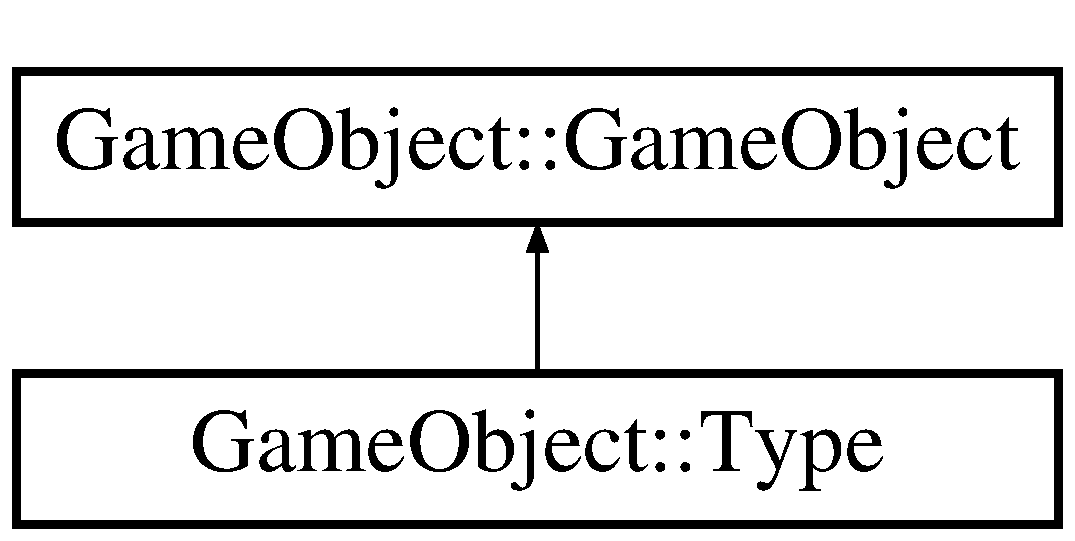
\includegraphics[height=2cm]{classGameObject_1_1Type}
\end{center}
\end{figure}
\subsection*{Public Member Functions}
\begin{DoxyCompactItemize}
\item 
\hypertarget{classGameObject_1_1Type_a62ae914c3017b69716212e83af59b02d}{
def {\bfseries \_\-\_\-init\_\-\_\-}}
\label{classGameObject_1_1Type_a62ae914c3017b69716212e83af59b02d}

\item 
\hypertarget{classGameObject_1_1Type_a7d8d0f7426d7df79fcc1e381b3686541}{
def {\bfseries validify}}
\label{classGameObject_1_1Type_a7d8d0f7426d7df79fcc1e381b3686541}

\item 
\hypertarget{classGameObject_1_1Type_ac1e4a727810e33a69eb691e5d06d23b2}{
def \hyperlink{classGameObject_1_1Type_ac1e4a727810e33a69eb691e5d06d23b2}{getId}}
\label{classGameObject_1_1Type_ac1e4a727810e33a69eb691e5d06d23b2}

\begin{DoxyCompactList}\small\item\em Unique Identifier. \item\end{DoxyCompactList}\item 
\hypertarget{classGameObject_1_1Type_a0130ebca6b9bcc12603ddc62d6d559d8}{
def \hyperlink{classGameObject_1_1Type_a0130ebca6b9bcc12603ddc62d6d559d8}{getName}}
\label{classGameObject_1_1Type_a0130ebca6b9bcc12603ddc62d6d559d8}

\begin{DoxyCompactList}\small\item\em The name of this type of robot. \item\end{DoxyCompactList}\item 
\hypertarget{classGameObject_1_1Type_a4609fc18dbf135b12ad9c92ff388bb17}{
def \hyperlink{classGameObject_1_1Type_a4609fc18dbf135b12ad9c92ff388bb17}{getMaxHealth}}
\label{classGameObject_1_1Type_a4609fc18dbf135b12ad9c92ff388bb17}

\begin{DoxyCompactList}\small\item\em The maximum amount of health for this type of robot. \item\end{DoxyCompactList}\item 
\hypertarget{classGameObject_1_1Type_a25e293b331ac205d8ded863f87b77afa}{
def \hyperlink{classGameObject_1_1Type_a25e293b331ac205d8ded863f87b77afa}{getDamage}}
\label{classGameObject_1_1Type_a25e293b331ac205d8ded863f87b77afa}

\begin{DoxyCompactList}\small\item\em The amount of damage this type of robot does when attacking. \item\end{DoxyCompactList}\item 
\hypertarget{classGameObject_1_1Type_a580b3d9dbb81cdd1954318800422db75}{
def \hyperlink{classGameObject_1_1Type_a580b3d9dbb81cdd1954318800422db75}{getRange}}
\label{classGameObject_1_1Type_a580b3d9dbb81cdd1954318800422db75}

\begin{DoxyCompactList}\small\item\em How far this type of robot can attack or heal from its edge. \item\end{DoxyCompactList}\item 
\hypertarget{classGameObject_1_1Type_a1b955c2cf04692c2613dddf8e19bdbf2}{
def \hyperlink{classGameObject_1_1Type_a1b955c2cf04692c2613dddf8e19bdbf2}{getMovitude}}
\label{classGameObject_1_1Type_a1b955c2cf04692c2613dddf8e19bdbf2}

\begin{DoxyCompactList}\small\item\em This value divided by the number of bots = maxSteps for this type of robot. \item\end{DoxyCompactList}\item 
\hypertarget{classGameObject_1_1Type_af813e0a11a084c09820a600cae8ac031}{
def \hyperlink{classGameObject_1_1Type_af813e0a11a084c09820a600cae8ac031}{getActitude}}
\label{classGameObject_1_1Type_af813e0a11a084c09820a600cae8ac031}

\begin{DoxyCompactList}\small\item\em This value divided by the number of bots = maxActions for this type of robot. \item\end{DoxyCompactList}\item 
\hypertarget{classGameObject_1_1Type_a8c1e9901918a6acccd7e45dc9527894f}{
def \hyperlink{classGameObject_1_1Type_a8c1e9901918a6acccd7e45dc9527894f}{getBuildRate}}
\label{classGameObject_1_1Type_a8c1e9901918a6acccd7e45dc9527894f}

\begin{DoxyCompactList}\small\item\em This value is used to determine how many turns it takes to build a robot and how much this type of robot heals for. \item\end{DoxyCompactList}\item 
\hypertarget{classGameObject_1_1Type_ae31f5db029f8213edf2386587655fec7}{
def {\bfseries \_\-\_\-str\_\-\_\-}}
\label{classGameObject_1_1Type_ae31f5db029f8213edf2386587655fec7}

\end{DoxyCompactItemize}
\subsection*{Public Attributes}
\begin{DoxyCompactItemize}
\item 
\hypertarget{classGameObject_1_1Type_a9ad3b17633de07c109b9cde37c9192a9}{
{\bfseries ptr}}
\label{classGameObject_1_1Type_a9ad3b17633de07c109b9cde37c9192a9}

\item 
\hypertarget{classGameObject_1_1Type_adbe374e9663c0869e0e29650fd63323d}{
{\bfseries iteration}}
\label{classGameObject_1_1Type_adbe374e9663c0869e0e29650fd63323d}

\item 
\hypertarget{classGameObject_1_1Type_a49dc9726276a22fa48d21f06baa19275}{
{\bfseries id}}
\label{classGameObject_1_1Type_a49dc9726276a22fa48d21f06baa19275}

\end{DoxyCompactItemize}


\subsection{Detailed Description}
A kind of robot. 

The documentation for this class was generated from the following file:\begin{DoxyCompactItemize}
\item 
GameObject.py\end{DoxyCompactItemize}

\hypertarget{classGameObject_1_1Unit}{
\section{GameObject::Unit Class Reference}
\label{classGameObject_1_1Unit}\index{GameObject::Unit@{GameObject::Unit}}
}


An object that exists on the grid.  


Inheritance diagram for GameObject::Unit:\begin{figure}[H]
\begin{center}
\leavevmode
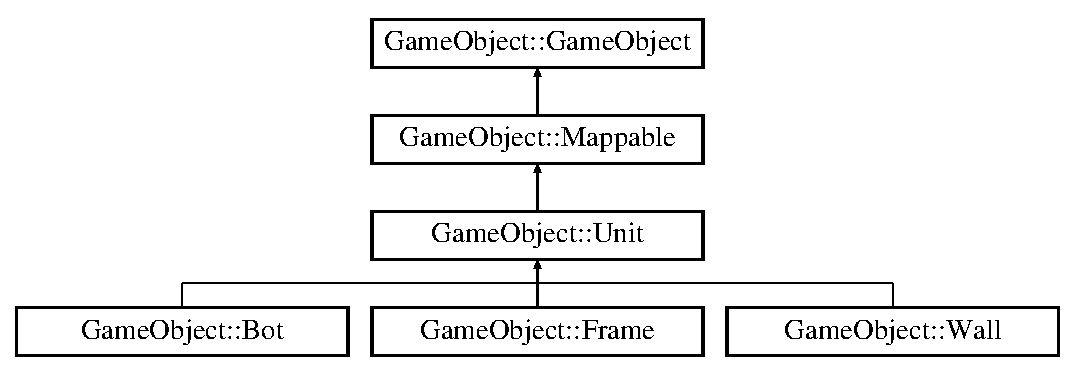
\includegraphics[height=4cm]{classGameObject_1_1Unit}
\end{center}
\end{figure}
\subsection*{Public Member Functions}
\begin{DoxyCompactItemize}
\item 
\hypertarget{classGameObject_1_1Unit_a29efd7d8ec0ee55b4cfd2a198c42eab5}{
def {\bfseries \_\-\_\-init\_\-\_\-}}
\label{classGameObject_1_1Unit_a29efd7d8ec0ee55b4cfd2a198c42eab5}

\item 
\hypertarget{classGameObject_1_1Unit_ab32e23a3a72c78ebae7270bba1f619b1}{
def \hyperlink{classGameObject_1_1Unit_ab32e23a3a72c78ebae7270bba1f619b1}{talk}}
\label{classGameObject_1_1Unit_ab32e23a3a72c78ebae7270bba1f619b1}

\begin{DoxyCompactList}\small\item\em Sends a message to be visualized when this unit is selected. \item\end{DoxyCompactList}\item 
\hypertarget{classGameObject_1_1Unit_ade3a9d46b4c71e305744a0ac4ea4bce5}{
def \hyperlink{classGameObject_1_1Unit_ade3a9d46b4c71e305744a0ac4ea4bce5}{getId}}
\label{classGameObject_1_1Unit_ade3a9d46b4c71e305744a0ac4ea4bce5}

\begin{DoxyCompactList}\small\item\em Unique Identifier. \item\end{DoxyCompactList}\item 
def \hyperlink{classGameObject_1_1Unit_a01711efd87c7e3e2a97066e9a5c50da5}{getX}
\begin{DoxyCompactList}\small\item\em The X position of the top left corner of this object. \item\end{DoxyCompactList}\item 
def \hyperlink{classGameObject_1_1Unit_a4d0c47deb0ddb19b9e2b195d8ca2f2ad}{getY}
\begin{DoxyCompactList}\small\item\em The Y position of the top left corner of this object. \item\end{DoxyCompactList}\item 
\hypertarget{classGameObject_1_1Unit_a492eeeaefbaada8b03c756d884c46978}{
def \hyperlink{classGameObject_1_1Unit_a492eeeaefbaada8b03c756d884c46978}{getOwner}}
\label{classGameObject_1_1Unit_a492eeeaefbaada8b03c756d884c46978}

\begin{DoxyCompactList}\small\item\em The owning player. \item\end{DoxyCompactList}\item 
\hypertarget{classGameObject_1_1Unit_aa2ed517e2aa409e708e05156a00c4e84}{
def \hyperlink{classGameObject_1_1Unit_aa2ed517e2aa409e708e05156a00c4e84}{getHealth}}
\label{classGameObject_1_1Unit_aa2ed517e2aa409e708e05156a00c4e84}

\begin{DoxyCompactList}\small\item\em How much health this unit currently has. \item\end{DoxyCompactList}\item 
\hypertarget{classGameObject_1_1Unit_a566b46c59ff8ceacb70b0c1a639aea26}{
def \hyperlink{classGameObject_1_1Unit_a566b46c59ff8ceacb70b0c1a639aea26}{getMaxHealth}}
\label{classGameObject_1_1Unit_a566b46c59ff8ceacb70b0c1a639aea26}

\begin{DoxyCompactList}\small\item\em The maximum amount of health this unit can ever have. \item\end{DoxyCompactList}\item 
\hypertarget{classGameObject_1_1Unit_aa4947e4f517074ddbf8e65f374f33c7b}{
def \hyperlink{classGameObject_1_1Unit_aa4947e4f517074ddbf8e65f374f33c7b}{getSize}}
\label{classGameObject_1_1Unit_aa4947e4f517074ddbf8e65f374f33c7b}

\begin{DoxyCompactList}\small\item\em The length of one side of this \hyperlink{classGameObject_1_1Unit}{Unit}. \item\end{DoxyCompactList}\item 
\hypertarget{classGameObject_1_1Unit_a80f9fbb90bcfc89ba78500bb3b83b223}{
def {\bfseries \_\-\_\-str\_\-\_\-}}
\label{classGameObject_1_1Unit_a80f9fbb90bcfc89ba78500bb3b83b223}

\end{DoxyCompactItemize}
\subsection*{Public Attributes}
\begin{DoxyCompactItemize}
\item 
\hypertarget{classGameObject_1_1Unit_aeed6c6641d9ab913c271e07ce91f66dc}{
{\bfseries ptr}}
\label{classGameObject_1_1Unit_aeed6c6641d9ab913c271e07ce91f66dc}

\item 
\hypertarget{classGameObject_1_1Unit_aa9e881997b25f4452c57074760815d63}{
{\bfseries iteration}}
\label{classGameObject_1_1Unit_aa9e881997b25f4452c57074760815d63}

\item 
\hypertarget{classGameObject_1_1Unit_a420650a7a0736e831568a65e7b377cd4}{
{\bfseries id}}
\label{classGameObject_1_1Unit_a420650a7a0736e831568a65e7b377cd4}

\end{DoxyCompactItemize}


\subsection{Detailed Description}
An object that exists on the grid. 

\subsection{Member Function Documentation}
\hypertarget{classGameObject_1_1Unit_a01711efd87c7e3e2a97066e9a5c50da5}{
\index{GameObject::Unit@{GameObject::Unit}!getX@{getX}}
\index{getX@{getX}!GameObject::Unit@{GameObject::Unit}}
\subsubsection[{getX}]{\setlength{\rightskip}{0pt plus 5cm}def GameObject::Unit::getX ( {\em self})}}
\label{classGameObject_1_1Unit_a01711efd87c7e3e2a97066e9a5c50da5}


The X position of the top left corner of this object. 

X is horizontal 

Reimplemented from \hyperlink{classGameObject_1_1Mappable_a3ae7d302c87c0a6f1e211a7584c3b807}{GameObject::Mappable}.



Reimplemented in \hyperlink{classGameObject_1_1Bot_a76521d97d7dcce093efbdd1926c75750}{GameObject::Bot}, \hyperlink{classGameObject_1_1Frame_aab513e4859fc8a9f5d5f1a6b47cb6df3}{GameObject::Frame}, and \hyperlink{classGameObject_1_1Wall_aa8d092fd75ef8372aacf4ece64521ea8}{GameObject::Wall}.

\hypertarget{classGameObject_1_1Unit_a4d0c47deb0ddb19b9e2b195d8ca2f2ad}{
\index{GameObject::Unit@{GameObject::Unit}!getY@{getY}}
\index{getY@{getY}!GameObject::Unit@{GameObject::Unit}}
\subsubsection[{getY}]{\setlength{\rightskip}{0pt plus 5cm}def GameObject::Unit::getY ( {\em self})}}
\label{classGameObject_1_1Unit_a4d0c47deb0ddb19b9e2b195d8ca2f2ad}


The Y position of the top left corner of this object. 

Y is vertical 

Reimplemented from \hyperlink{classGameObject_1_1Mappable_af7b558a1be2dc80d1aa78f306e226c10}{GameObject::Mappable}.



Reimplemented in \hyperlink{classGameObject_1_1Bot_a5e193704cae24529a6e6f00fd9a1447f}{GameObject::Bot}, \hyperlink{classGameObject_1_1Frame_abf564d6f986b8e9d2a83838691c591f9}{GameObject::Frame}, and \hyperlink{classGameObject_1_1Wall_ac87b620714dfacc5ac12ca6078a91460}{GameObject::Wall}.



The documentation for this class was generated from the following file:\begin{DoxyCompactItemize}
\item 
GameObject.py\end{DoxyCompactItemize}

\hypertarget{classGameObject_1_1Wall}{
\section{GameObject::Wall Class Reference}
\label{classGameObject_1_1Wall}\index{GameObject::Wall@{GameObject::Wall}}
}


A pile of hard stuff that is in the way.  


Inheritance diagram for GameObject::Wall:\begin{figure}[H]
\begin{center}
\leavevmode
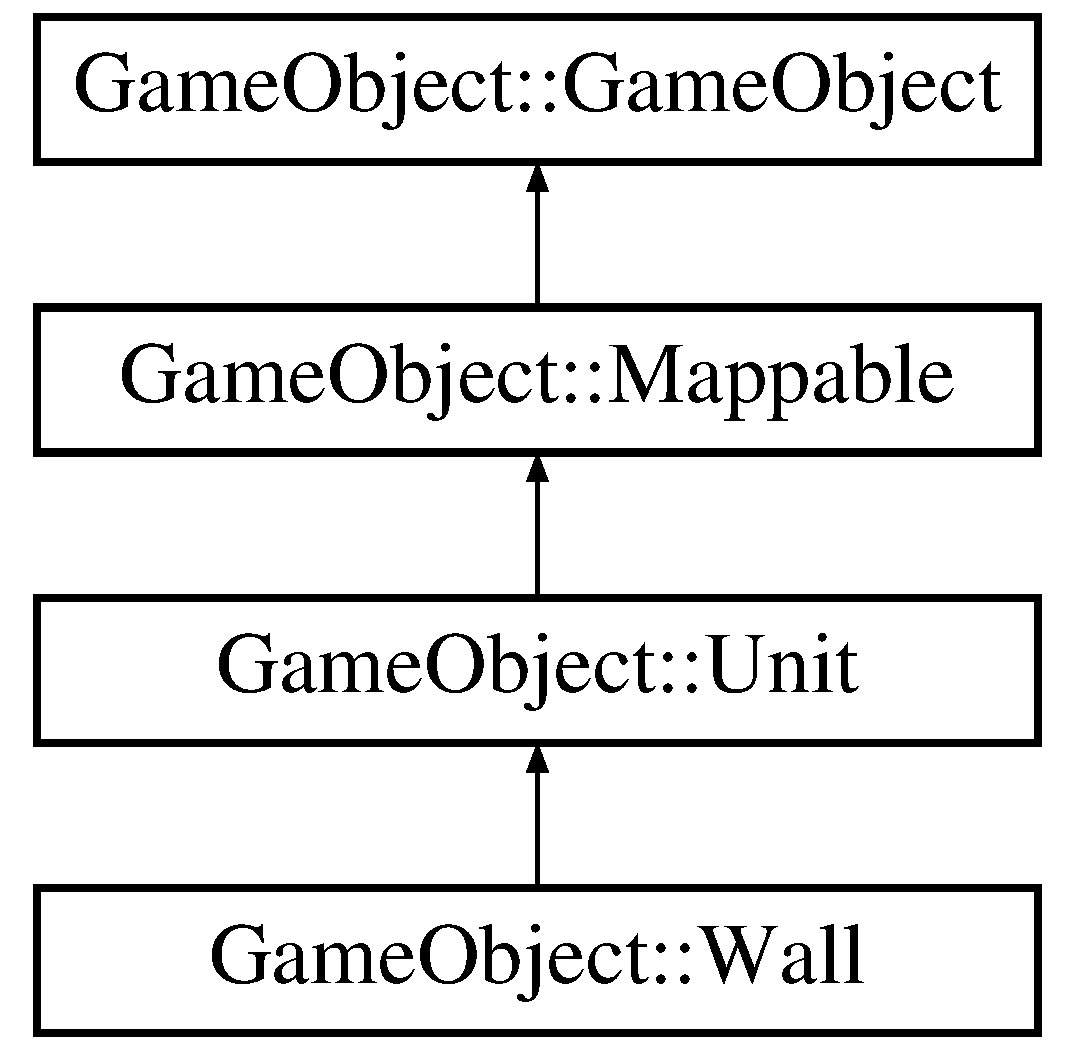
\includegraphics[height=4cm]{classGameObject_1_1Wall}
\end{center}
\end{figure}
\subsection*{Public Member Functions}
\begin{DoxyCompactItemize}
\item 
\hypertarget{classGameObject_1_1Wall_a216c45c047f96de9ef04caf5efe57fa1}{
def {\bfseries \_\-\_\-init\_\-\_\-}}
\label{classGameObject_1_1Wall_a216c45c047f96de9ef04caf5efe57fa1}

\item 
\hypertarget{classGameObject_1_1Wall_ad6dadcc822c606f8cd60ab8925822097}{
def {\bfseries validify}}
\label{classGameObject_1_1Wall_ad6dadcc822c606f8cd60ab8925822097}

\item 
\hypertarget{classGameObject_1_1Wall_aaff85bff56a8e19ea844573773e1936b}{
def \hyperlink{classGameObject_1_1Wall_aaff85bff56a8e19ea844573773e1936b}{talk}}
\label{classGameObject_1_1Wall_aaff85bff56a8e19ea844573773e1936b}

\begin{DoxyCompactList}\small\item\em Sends a message to be visualized when this unit is selected. \item\end{DoxyCompactList}\item 
\hypertarget{classGameObject_1_1Wall_afbaaf0e2bde922af009a6f4685ccc589}{
def \hyperlink{classGameObject_1_1Wall_afbaaf0e2bde922af009a6f4685ccc589}{getId}}
\label{classGameObject_1_1Wall_afbaaf0e2bde922af009a6f4685ccc589}

\begin{DoxyCompactList}\small\item\em Unique Identifier. \item\end{DoxyCompactList}\item 
def \hyperlink{classGameObject_1_1Wall_aa8d092fd75ef8372aacf4ece64521ea8}{getX}
\begin{DoxyCompactList}\small\item\em The X position of the top left corner of this object. \item\end{DoxyCompactList}\item 
def \hyperlink{classGameObject_1_1Wall_ac87b620714dfacc5ac12ca6078a91460}{getY}
\begin{DoxyCompactList}\small\item\em The Y position of the top left corner of this object. \item\end{DoxyCompactList}\item 
\hypertarget{classGameObject_1_1Wall_ad95dd3f80c773e982263873044771f31}{
def \hyperlink{classGameObject_1_1Wall_ad95dd3f80c773e982263873044771f31}{getOwner}}
\label{classGameObject_1_1Wall_ad95dd3f80c773e982263873044771f31}

\begin{DoxyCompactList}\small\item\em The owning player. \item\end{DoxyCompactList}\item 
\hypertarget{classGameObject_1_1Wall_abacbb0b4d5729c993040b0f6b8ae3069}{
def \hyperlink{classGameObject_1_1Wall_abacbb0b4d5729c993040b0f6b8ae3069}{getHealth}}
\label{classGameObject_1_1Wall_abacbb0b4d5729c993040b0f6b8ae3069}

\begin{DoxyCompactList}\small\item\em How much health this unit currently has. \item\end{DoxyCompactList}\item 
\hypertarget{classGameObject_1_1Wall_a7fd11d3b45f2a4c4ce9c4ee1cdb3a508}{
def \hyperlink{classGameObject_1_1Wall_a7fd11d3b45f2a4c4ce9c4ee1cdb3a508}{getMaxHealth}}
\label{classGameObject_1_1Wall_a7fd11d3b45f2a4c4ce9c4ee1cdb3a508}

\begin{DoxyCompactList}\small\item\em The maximum amount of health this unit can ever have. \item\end{DoxyCompactList}\item 
\hypertarget{classGameObject_1_1Wall_a1340a600c968946cdc328fa7296f88fd}{
def \hyperlink{classGameObject_1_1Wall_a1340a600c968946cdc328fa7296f88fd}{getSize}}
\label{classGameObject_1_1Wall_a1340a600c968946cdc328fa7296f88fd}

\begin{DoxyCompactList}\small\item\em The length of one side of this \hyperlink{classGameObject_1_1Unit}{Unit}. \item\end{DoxyCompactList}\item 
\hypertarget{classGameObject_1_1Wall_ad10be1aaaadeffa34b4903a2b4d7d1de}{
def {\bfseries \_\-\_\-str\_\-\_\-}}
\label{classGameObject_1_1Wall_ad10be1aaaadeffa34b4903a2b4d7d1de}

\end{DoxyCompactItemize}
\subsection*{Public Attributes}
\begin{DoxyCompactItemize}
\item 
\hypertarget{classGameObject_1_1Wall_aca77f48e399779816107f66d08db19ea}{
{\bfseries ptr}}
\label{classGameObject_1_1Wall_aca77f48e399779816107f66d08db19ea}

\item 
\hypertarget{classGameObject_1_1Wall_aeec50205498a30561831f88ec5816c9a}{
{\bfseries iteration}}
\label{classGameObject_1_1Wall_aeec50205498a30561831f88ec5816c9a}

\item 
\hypertarget{classGameObject_1_1Wall_ac238c673f341e4e5e51e811e4296c12b}{
{\bfseries id}}
\label{classGameObject_1_1Wall_ac238c673f341e4e5e51e811e4296c12b}

\end{DoxyCompactItemize}


\subsection{Detailed Description}
A pile of hard stuff that is in the way. 

\subsection{Member Function Documentation}
\hypertarget{classGameObject_1_1Wall_aa8d092fd75ef8372aacf4ece64521ea8}{
\index{GameObject::Wall@{GameObject::Wall}!getX@{getX}}
\index{getX@{getX}!GameObject::Wall@{GameObject::Wall}}
\subsubsection[{getX}]{\setlength{\rightskip}{0pt plus 5cm}def GameObject::Wall::getX ( {\em self})}}
\label{classGameObject_1_1Wall_aa8d092fd75ef8372aacf4ece64521ea8}


The X position of the top left corner of this object. 

X is horizontal 

Reimplemented from \hyperlink{classGameObject_1_1Unit_a01711efd87c7e3e2a97066e9a5c50da5}{GameObject::Unit}.

\hypertarget{classGameObject_1_1Wall_ac87b620714dfacc5ac12ca6078a91460}{
\index{GameObject::Wall@{GameObject::Wall}!getY@{getY}}
\index{getY@{getY}!GameObject::Wall@{GameObject::Wall}}
\subsubsection[{getY}]{\setlength{\rightskip}{0pt plus 5cm}def GameObject::Wall::getY ( {\em self})}}
\label{classGameObject_1_1Wall_ac87b620714dfacc5ac12ca6078a91460}


The Y position of the top left corner of this object. 

Y is vertical 

Reimplemented from \hyperlink{classGameObject_1_1Unit_a4d0c47deb0ddb19b9e2b195d8ca2f2ad}{GameObject::Unit}.



The documentation for this class was generated from the following file:\begin{DoxyCompactItemize}
\item 
GameObject.py\end{DoxyCompactItemize}

\printindex
\end{document}
